\chapter{\ac{yolo} Model for Video Analysis}
\label{chapter:yolo}

\newenvironment{yolo}
{\quote\itshape}
{\endquote}

\begin{yolo}
    This chapter explores the evolution of the \ac{yolo} family of models, with a particular focus on the capabilities
    of \ac{yolo}v5. Additionally, it outlines the process of dataset creation, highlighting the steps taken to 
    ensure high-quality data for training and evaluating the model 
    in video analysis applications.
\end{yolo}

\subsection{\ac{yolo} Versions Overview}
The figure \ref{fig:yolo-versions} describes the timeline of \ac{yolo} versions, highlighting the 
progression and key developments from its inception to the latest versions. The timeline begins with YOLOv1 
introduced in 2015 and extends to YOLOv8 and YOLO-NAS in 2023.

\begin{figure}[h]
    \centering 
    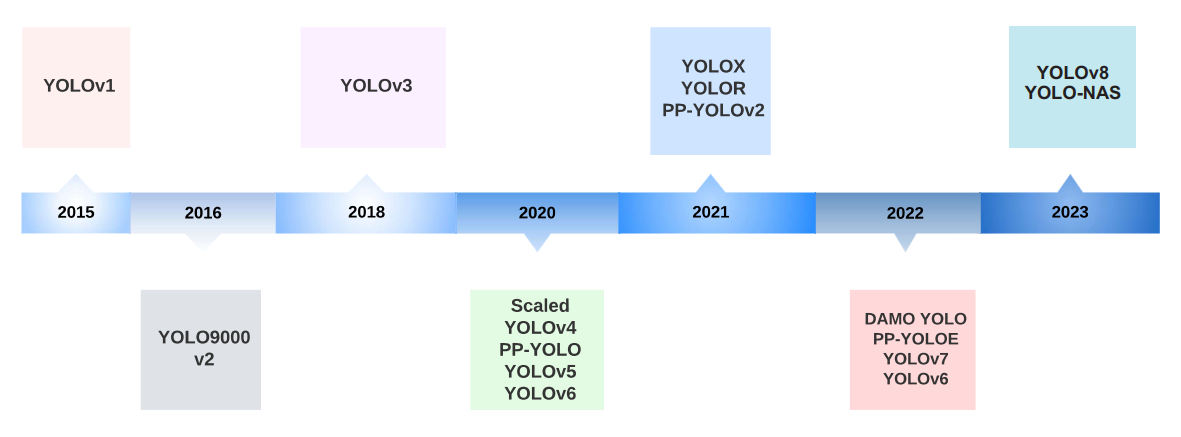
\includegraphics[width=0.75\textwidth]{figs/yolo-versions.png} 
    \caption{\ac{yolo} Versions Timeline \cite{rfc50}}
    \label{fig:yolo-versions}
\end{figure}

\citet{rfc51} work shows a summary of the key improvements and characteristics of each YOLO version:
\begin{itemize}
    \item YOLOv1 (2015): first real-time object detection system with a single convolutional network pass; 
    \item YOLOv2 (2017): this version included higher resolution and anchor boxes. It contains 5 max-pooling layers, 
    implemented with Darknet, and has 19 convolutional layers;
    \item YOLOv3 (2018): focused on improving performance on smaller objects, it increased the number of layers to 106;
    \item YOLOv4 (2020): known for optimal speed and accuracy, it features 53 convolutional layers of specific sizes;
    \item YOLOv5 (2020): introduced mosaic augmentation and consists of 80 classes of 3 parts;
    \item YOLOv6 (2021): includes architectural improvements, although the total number of layers is not fixed;
    \item YOLOv7 (2021): designed for faster inference and greater accuracy, the total number of layers is also not fixed;
    \item YOLOv8 (2023): offers improved adaptive training, customizable architecture, and advanced data augmentation, 
    with the total number of layers not fixed.
\end{itemize}

\ac{yolo}v5 was chosen for its balance of speed and accuracy, building on the strengths of previous \ac{yolo} versions to 
enhance detection performance.  Its stability and maturity have been proven through extensive real-world testing 
and a strong support ecosystem, making it a reliable choice. Besides, prior knowledge and experience with this version 
facilitated smoother integration and application.

While newer versions may offer specific improvements, they do not have the same level of reliability and 
resource availability as \ac{yolo}v5, making it the preferred option for reliable and efficient object detection tasks.
A good point to consider for the future is to evaluate the integration and use of a newer version. Testing it and 
applying it in the application could bring better results.

\subsection{\ac{yolo}v5 Model Overview}
The \ac{yolo}v5 architecture, as depicted in the diagram \ref{fig:yolov5-architecture}, is organized into 
three primary sections: the Backbone, the Neck, and the Head.

\begin{figure}[h]
    \centering 
    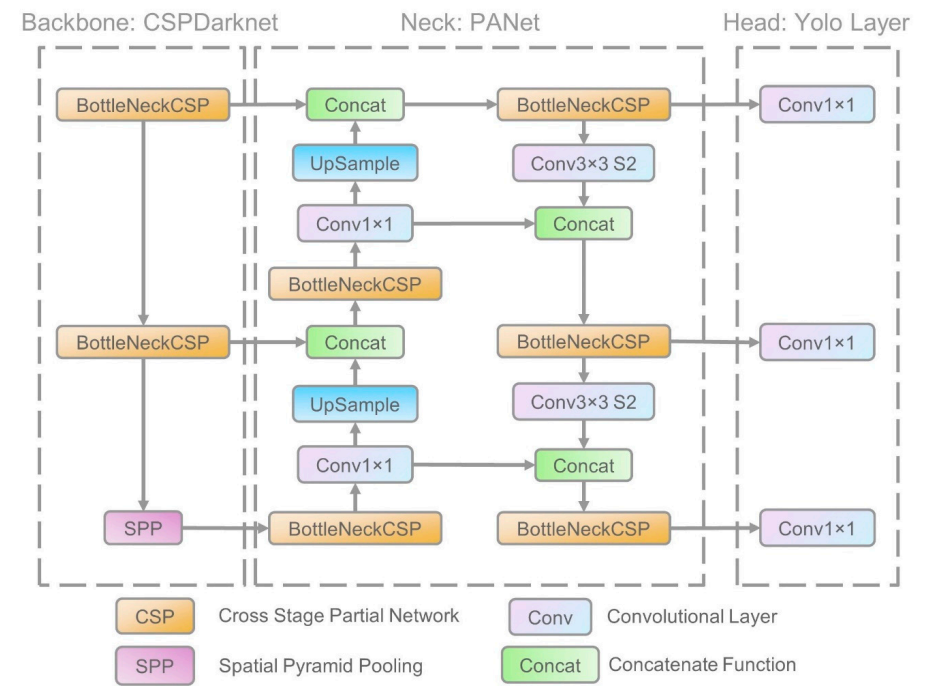
\includegraphics[width=0.65\textwidth]{figs/yolov5-architecture2.png} 
    \caption{YOLOv5 Architecture \cite{rfc49}}
    \label{fig:yolov5-architecture}
\end{figure}

The backbone of the network, CSPDarknet, is essential for the initial processing and feature extraction from raw input data.
It uses multiple BottleNeckCSP blocks, which are crucial to the Cross Stage Partial Network (CSPNet) \cite{rfc49}.

CSPNet is designed to address a common issue in large-scale neural networks - the redundancy of gradient information. 
It occurs when the same or similar gradient information is repeatedly used to update the network parameters, even though it does not contribute
new or valuable insights to the learning process.
Gradients are essential for adjusting the network during training, providing the necessary information to update 
the network's parameters, however, when redundant, they can slow the process.

CSPNet, represented on the diagram \ref{fig:cspnet}, addresses this issue by splitting the feature map of layers 
into parts at various stages within the network.
Using this strategy, split and merge, reduces the redudancy of the gradiant flow
 through the network, leading to more efficient 
learning processes. 

%As a result, networks utilizing CSPNet can achieve faster training times and require fewer 
%computational resources.

\begin{figure}[h]
    \centering 
    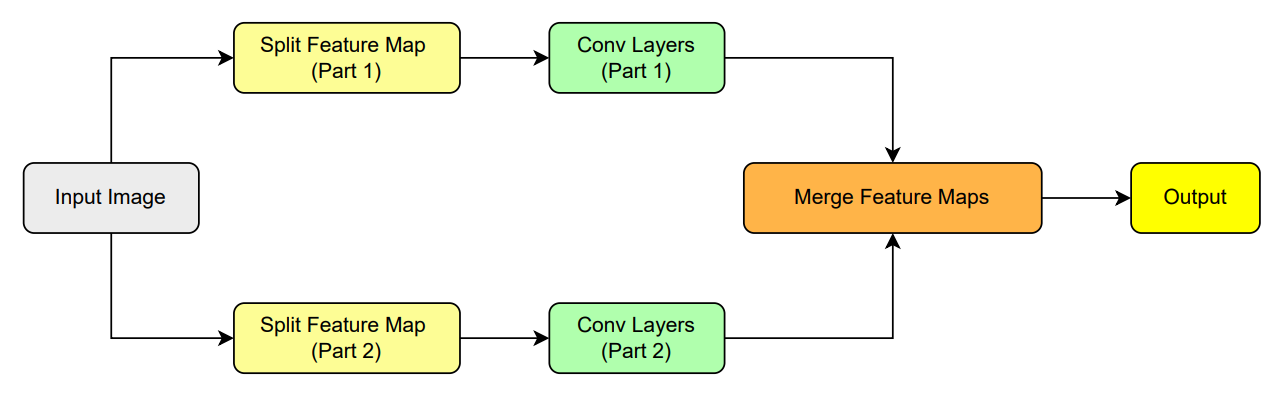
\includegraphics[width=0.75\textwidth]{figs/spnet.png} 
    \caption{CSPNet - Cross Stage Partial Network}
    \label{fig:cspnet}
\end{figure}

Feature extraction in this context involves using convolutional, pooling, and bottleneck layers to 
transform the raw input image into a set of feature maps. These maps encode essential visual information 
such as edges, textures, and other significant patterns that are pertinent for detecting objects.

Following the backbone, the Neck of the \ac{yolo}v5 architecture features the Path Aggregation Network (PANet). PANet 
enhances the feature pyramid network (FPN) with a strong bottom-up pathway, which improves the propagation and 
utilization of lower-level features across the network. This structure helps in better localization and detection 
accuracy, particularly for varied object sizes.

An FPN is crucial for constructing a pyramid of feature maps at multiple scales, allowing the network to detect 
objects effectively across different sizes. It does this by integrating semantic information from deep, coarse 
resolution feature maps with finer-resolution features from earlier layers through lateral connections and top-down 
pathways. This combination ensures that both high-level and low-level features contribute to the final detections.

\begin{figure}[h]
    \centering 
    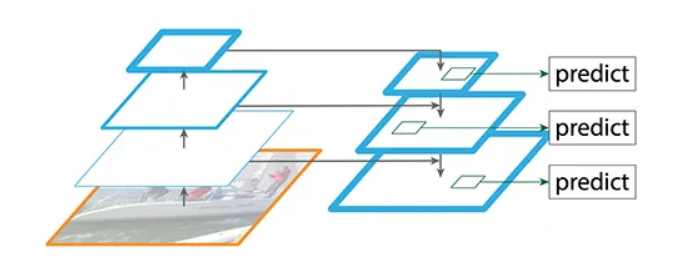
\includegraphics[width=0.6\textwidth]{figs/fpn.png} 
    \caption{Feature Pyramid Network}
    \label{fig:fpn}
\end{figure}

The final section is the \ac{yolo} Layer, which forms the detection head of the network. This layer processes the 
enriched feature maps to predict bounding boxes, object classes, and confidence scores.

\subsection{Dataset Proposed} 
The main purpose of our work is to detect firewarms and knifes (objets), however different tasks must be performed: 
select the dataset, train the dataset (with diferent configurations) and test the model under new test data. Therefore, 
the outcome of these tasks is a model to be used as part of our system.
Initially, to select our dataset we conduct a search based on the following parameters:
\begin{itemize}
    \item datasets annotated that contains images related to our domain;
    \item available for download;
    \item datasets used on scientific papers (not mandatory).
\end{itemize}

The datasets discovered that fullfill these parameters are:

\begin{itemize}
    \item DaSCI Dataset \cite{rfc29}: includes images of exposed weapons, specifically knives and handguns, along with various 
    random objects. Originally containing six different classes, it was restructured to include only two categories: 
    'knife' and 'weapons';
    \item Mock Attack Dataset \cite{rfc45}: images captured from three strategically positioned surveillance cameras in corridors 
    and an entrance, this dataset offers multiple viewing angles of scenarios where individuals are wielding weapons. 
    The images were annotated at a rate of two frames per second;
    \item Action Recognition and Object Detection Dataset \cite{rfc52}: several videos categorized into three types: no guns, handguns, 
    and machine guns, this dataset required significant modifications. The annotations were initially in JSON 
    format and had to be converted into .txt format compatible with \ac{yolo}v5 \footnote{\url{https://github.com/pedromonteiro01/yolo-utils/blob/main/json\_to\_txt\_annotations.py}}. Additionally, video frames were extracted 
    to form a static image dataset suitable for the training process.
\end{itemize}

Next, we performed the train and test. Figure \ref{fig:dataset-mq} describe the pipeline or trainning  and testing the selected dataset. 

\begin{figure}[h]
    \centering 
    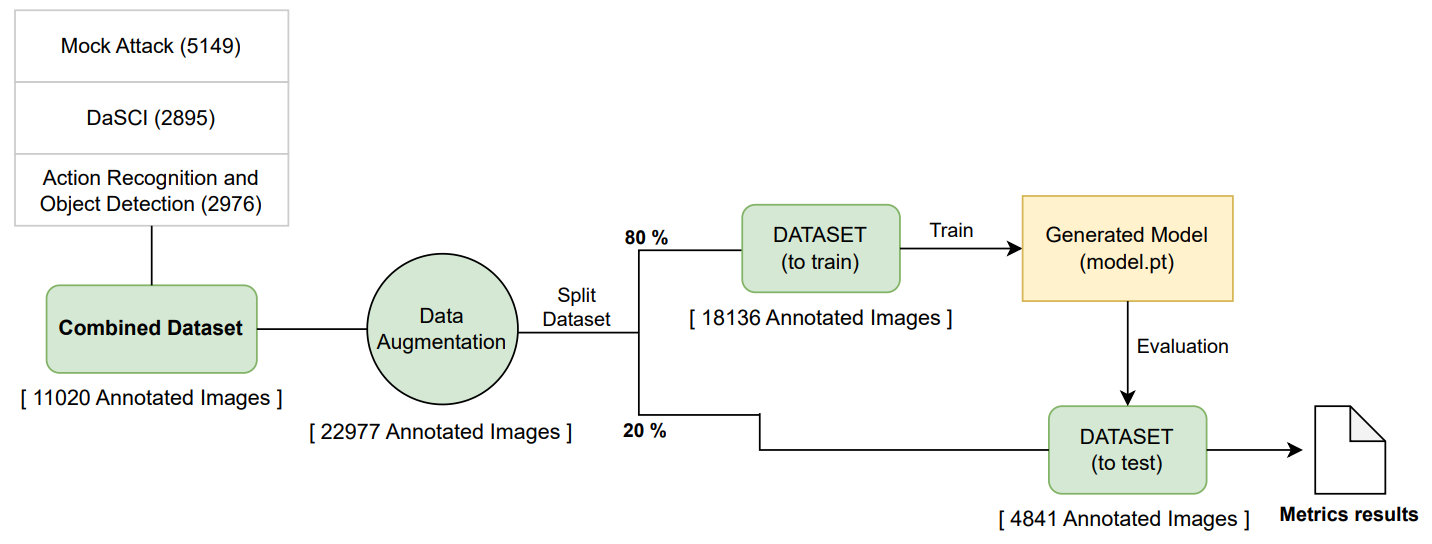
\includegraphics[width=0.75\textwidth]{figs/dataset-creation3.png} 
    \caption{Dataset Creation Steps}
    \label{fig:dataset-mq}
\end{figure}


First, the dataset is submited into data augmentation task divided into two subtasks: in the first task, images were 
randomly blurred and rotated to produce some variability; in a second task, images underwent brightness adjustments,
resulting in sets of images that were either darker or lighter \footnote{\url{https://github.com/pedromonteiro01/yolo-utils/blob/main/augment.py}}.

The dataset resulted has a total of 22977 images. These images were divided into 
80\% to train, and 20\% to test. The model generation were submited to a fine tunning to achieve the best metrics results.
